\section{Il Modello Standard}
In questa sezione verrà studiato quello che è il modello standard delle particelle, ovvero tutte le leggi date per confermate e che costituiscono la base degli studi fisici. 
Esistono delle teorie con evidenze sperimentali che vanno oltre a questo modello ma sono spesso teorie non ancora totalmente sviluppate che verranno implementate.
Lo studio del modello standard sarà approfondito nei corsi della magistrale ma è giusto che uno studente della triennale abbia comunque un'idea generale di quello che è.

%nuova sezione------------------------------------------------------------------------------ 
\subsection{Fisica degli acceleratori di particelle}
La conoscenza della fisica degli acceleratori è essenziale per ogni tipo di fisico in quanto ha applicazioni in ogni campo fisico.
Ne approfondiamo quindi quelli che sono i fondamenti e le grandezze base per poter avere un'idea più chiara del loro funzionamento.

Per capire la grande applicabilità di questi strumenti, attualmente al mondo sono attivi $15000$ acceleratori di cui: $8500$ con applicazioni industriali, $5500$ con applicazioni mediche e $1000$ con applicazioni in ricerca (di cui $100$ usati per la fisica nucleare e subnucleare).
L'attenzione mondiale alla fisica nucleare cambiò radicalmente prima e dopo la seconda guerra mondiale e anche gli acceleratori sono figli dell'aumento dell'interesse a questi ambiti.
Già a Rutherford dopo i suoi studi era chiaro che l'accelerazione di particelle sarebbe stato il passo successivo per la scoperta e l'approfondimento di questa nuova fisica.
Solo avendo il controllo della quantità ed energia di particelle si sarebbe potuto infatti ottenere una maggiore risoluzione nello studio del nucleo.

I parametri che caratterizzano gli acceleratori sono sostanzialmente l'energia e la luminosità.

\paragraph{Energia}. 

\'E importante conoscere l'energia perché la risoluzione con la quale possiamo risolvere un bersaglio dipende dalla lunghezza d'onda della sonda con la quale bombardiamo l'oggetto in analisi.
Prendendo un oggetto di raggio R, la lunghezza d'onda della sonda dovrà essere
\begin{equation}
\begin{split}
\lambda=\frac{h}{p}&<2R\\
2\pi \frac{\hbar c}{pc}&<2R
\end{split}
\end{equation}
Vuol dire che se vogliamo risolvere una struttura di dimensione $2R$ dobbiamo avere un fascio di energia
\begin{equation}
pc\simeq E>2\pi\frac{\hbar c}{2R}
\end{equation}
Inserendo quindi un po' di dimensioni, se vogliamo per esempio studiare il protone ($r=1fm$) serve un energia pari a 
\begin{equation}
E=pc=600MeV
\end{equation}
Se per esempio invece volessimo studiare i quark($r=10^{-4}fm$) allora l'energia sarà
\begin{equation}
E\simeq 6TeV
\end{equation}

Un altro motivo per cui è essenziale l'energia negli acceleratori deriva dalla famosa formula di Einstein
\begin{equation}
E=mc^2
\end{equation}
Che prevede la convertibilità tra massa ed energia.
Nella sezione precedente abbiamo infatti visto come sia possibile generare energia trasformando della massa.
Se questo è vero allora sarà vero anche il contrario, infatti è stato visto negli acceleratori che da scontri tra particelle altamente energetiche è possibile generare nuove particelle.
Per cui un grande utilizzo di questi apparati deriva proprio dalla necessità di generare particelle che sono state crucciali nello studio dell'evoluzione dell'universo che però sono ormai decadute per il basso tempo di decadimento.
Per dire proprio a questo scopo è stato costruito l'LHCb del Cern.

\paragraph{Metodi di collisione}
Esistono due modi per studiare le collisioni tra particelle: il metodo con il collisore e la collisione su bersaglio fisso.
Nel caso di collider (metodo del collisore) si sfruttano due fasci il che porta a delle energie nel centro di massa molto elevate (è quindi adatto alla produzione di nuove particelle).
Nel caso invece del bersaglio fisso l'energia è più bassa, ergo si fa più fatica a produrre nuove particelle, è favorita però la \emph{luminosità}.

Facciamo quindi delle stime sui due metodi
\begin{itemize}
\item Caso del collisore simmetrico.

Si consideri di avere due fasci paralleli e opposti in collisione, per semplicità adotteremo la semplificazione $\hbar=c=1$.
Il quadrivettore legato alla particella 1 è dato da
\begin{equation}
p_1*=(E_1*,\bar{p})
\end{equation}
(con asterisco indico le quantità misurate nel centro di massa).
Siccome i due fasci hanno lo stesso momento contropropagante è utile porsi nel sistema di riferimento del centro di massa , inoltre le due quantità di moto saranno identiche per cui non serve distinguere tra $\bar{p_1}$ e $\bar{p_2}$.
\begin{equation}
p_2*=(E_2*,-\bar{p})
\end{equation}
Si sa dalla meccanica relativistica che il quadrato del quadrivettore è un invariante relativistico
\begin{equation}
{p_1*}^2=E_1*-\bar{p}^2=m_1^2\\hspace{0.5cm}{p_2*}^2=E_2*-\bar{p}^2=m_2^2
\end{equation}
L'energia nel centro di massa è la somma dei quadrivettori al quadrato
\begin{equation}
\begin{split}
&s=(p_1*+p_2*)2=(E_1*+E_2*, \bar{p}-\bar{p})^2\\
&\to E_{CM}=\sqrt{s}=E_1*+E_2*
\end{split}
\end{equation}
Suppongo che il collider è simmetrico e che le particelle scontrate siano in entrambi i casi protoni (quindi di massa $m_p$).
L'energia di ogni fascio sarà
\begin{equation}
E_1*=m_1+T_{cm}=m_p+T_{cm}
\end{equation}
L'energia invece del centro di massa corrisponde a 
\begin{equation}
\sqrt{s}=E_{cm}=2m_p+2T_{cm}
\end{equation}
Quello che ci interessa è che se suppongo che l'energia nel centro di massa sia molto maggiore della massa del protone ($T_{cm}\gg m_p$), ottengo
\begin{equation}
T_{cm}=\frac{\sqrt{s}}{2}\to \sqrt{s}=2T_{cm}
\end{equation}
Quello che ci interessa è che in un collider l'energia nel centro di massa è linearmente dipendente dall'energia cinetica nel centro di massa.
Questo è importante perché quello che voglio creare nel centro di massa sono nuove particelle e così posso controllarne l'energia.

Il collider è un concetto molto complicato in quanto non è banale far scontrare due fasci, bisogna considerare che le dimensioni dei fasci infatti sono dell'ordine del millimetro e l'acceleratore è spesso lungo centinaia di metri.

Supponiamo di far scontrare due protoni e di voler creare un pione, particella costituita da un quark ed un anti quark.
\begin{equation}
pp\to pp\pi^0
\end{equation}
La massa di un pione è di 
\begin{equation}
m_{\pi^0}\simeq 130MeV/c^2
\end{equation}
L'energia dei due fasci per la formazione di un pione deve essere uguale a 
\begin{equation}
s_{cm}=(2m_pmm_{\pi^0})^2
\end{equation}
L'energia cinetica delle particelle deve soddisfare la condizione
\begin{equation}
2m_p+2T_{cm}\ge 2m_p+m_{\pi^0}
\end{equation}
e quindi essere
\begin{equation}
T_{cm}\ge \frac{m_{\pi^0}}{2}=67,5MeV
\end{equation}
L'energia cinetica richiesta per ogni fascio sarà quindi sempre pari alla metà dell'energia di massa della singola particella.
Questo si ottiene in quanto dobbiamo considerare che il centro di massa sarà sempre uguale.

\item Caso del bersaglio fisso.

Nel sistema di riferimento del laboratorio abbiamo che i due quadrivettori saranno 
\begin{equation}
\begin{split}
p_1&=(E_1,\bar{p_1}\\
p_2&=(m_2,0)
\end{split}
\end{equation}
Nel centro di massa il quadrivettore energia è 
\begin{equation}
\begin{split}
s&=[(E_1+m_2)^2-(\bar{p_2}+0)^2]\\
&=E_1^2+2E_1m_2+m_2^2-\bar{p_1}^2\\
&=m_1^2-+m_2^2+2E_1m_2
\end{split}
\end{equation}
A questo punto faccio le stesse considerazioni del collider, suppongo che le due particelle coincidano ($m_1=m_2=m_p$) e che l'energia della prima particella sia
\begin{equation}
E_1=m_1+T^{lab}
\end{equation}
ottengo quindi 
\begin{equation}
\begin{split}
s & =m_p^2 + m_p^2 + 2(m_p+T^{lab})m_p\\
\sqrt{s}&=\sqrt{4m_p^2+2T^{lab}m_p}
\end{split}
\end{equation}
Se mi pongo nella condizione in cui $T^{lab}\gg m_p$ ottengo
\begin{equation}
\sqrt{s}=\sqrt{2m_pT^{lab}}
\end{equation}

La differenza con il caso precedente è immediata, in un esperimento a bersaglio fisso l'energia nel centro di massa cresce linearmente con $\sqrt{T^{lab}}$.
Se volessi creare un pione con questa configurazione dovrei richiedere un'energia di soglia
\begin{equation}
\begin{split}
T^{lab}_{Th}&=\frac{s_{Th}-4m_p^2}{2m_p}\\
s_{Th}&=(2m_p+2m_{\pi^0})^2\\
T^{lab}_{Th}&=\frac{(2m_p+2m_{\pi^0})^2-4m_p^2}{2m_p}=280MeV
\end{split}
\end{equation}
Questo è solo un esempio per capire la differenza tra i due tipi di acceleratore.
\end{itemize}

\paragraph{Luminosità}
La luminosità $L$ corrisponde al numero di eventi (collisioni) per unità di area al secondo, è una grandezza importante perché se voglio calcolare il rate di eventi di un certo tipo 
\begin{equation}
R=\sigma L
\end{equation}
dove $\sigma$ è la sezione d'urto.

Per esempio nel Lep, che è stata la macchina progenitrice dell'LHC (funzionante tramite leptoni) e con cui si è studiato il modello standard, la produzione di coppie $W^+, W^-$ era di $\sigma=15pb$ e la luminosità (che si misura in numero di particelle su centimetro quadro al secondo) era di $L=10^{32}\cdot/cm^2s$.
Il che restituiva un rate di coppie pari a 
\begin{equation}
\frac{dW^+W^-}{dt}=15\times 10^{-12}\times 10^{-28}m^2\cdot 10^{32}\frac{1}{cm^2s}=1,5\times 10^{-3}\frac{eventi}{s}
\end{equation}
Si verificavano quindi un paio di eventi ogni ora.

La luminosità integrata nel tempo è una quantità che serve per capire per quanto tempo ho la necessità di sfruttare una strumentazione
\begin{equation}
L=\int Ldt
\end{equation}

La luminosità nel caso del collider si calcola come
\begin{equation}
L=\frac{nfN_1N_2}{A}
\end{equation}
dove $n$ è il numero di bunches (le particelle solitamente non sono distribuite uniformemente nei fasci a causa dei metodi sfruttati per collimare i fasci, vengono invece distribuite in pacchetti), $N_1, N_2$ sono il numero di particelle per bunch (ce ne sono due perché abbiamo due fasci e non sempre sono fasci uguali), $f$ è la frequenza di rivoluzione e $A$ è la sezione del fascio.
\'E intuitivo che per aumentare la luminosità dobbiamo rendere il fascio più piccolo possibile.

Nel caso del bersaglio fisso la luminosità è data da
\begin{equation}
L=\Phi_a N_b
\end{equation}
dove $\Phi_a$ è l'intensità di particelle del fascio e $N_b$ è il numero di particelle nel bersaglio.
L'intensità di particelle del fascio è uguale al numero di particelle al secondo diviso l'area
\begin{equation}
\Phi_a=\frac{N_a(s)}{A}
\end{equation}
che può anche essere scritta come la densità di particelle per unità di volume per la velocità delle particelle stesse
\begin{equation}
L=n_a v_a
\end{equation}
Mentre il numero di particelle del bersaglio è uguale alla densità delle particelle del bersaglio per lo spessore per l'area interessata del fascio
\begin{equation}
N_b=n_bd\cdot A
\end{equation}
La luminosità è quindi riscrivibile come
\begin{equation}
L=N_an_bd=n_av_aN_b
\end{equation}

%nuova sezione-----------------------------------------------------------------------------
\subsection{Tipi di Acceleratore}
Gli acceleratori si possono suddividere in due grandi categorie: acceleratori lineari e circolari.
\paragraph{Acceleratori Lineari}
Sono acceleratori elettrostatici ossia in questi acceleratori l'accelerazione avviene tramite una differenza di potenziale elettrostatico. 
In questa categoria sono inclusi gli acceleratori: 
\begin{itemize}
\item Van de Graaf
\item Cockrof-Walton
\item Tandem
\item il LINAC.
\end{itemize}
Il limite di questi acceleratori sta nel fatto che utilizzano un'unica differenza di potenziale, il che pone un limite a ciò che si può creare infatti le differenze di potenziale sono limitate dalla rottura del dielettrico.
Sono i primi che sono stati utilizzati e i massimi campi che si riesce a creare nel vuoto sono di $6-7MeV/m$

\paragraph{Acceleratori circolari}
Questi acceleratori ovviano al limite della differenza di potenziale facendo passare la particella più volte per la stessa differenza di potenziale facendo bastare così una piccola differenza di potenziale ben posta.
Di questi fanno parte:
\begin{itemize}
\item ciclotrone
\item betatrone
\item sincrotrone
\end{itemize}

\paragraph{Van De Graaf}
\begin{figure}[h]
\centering 
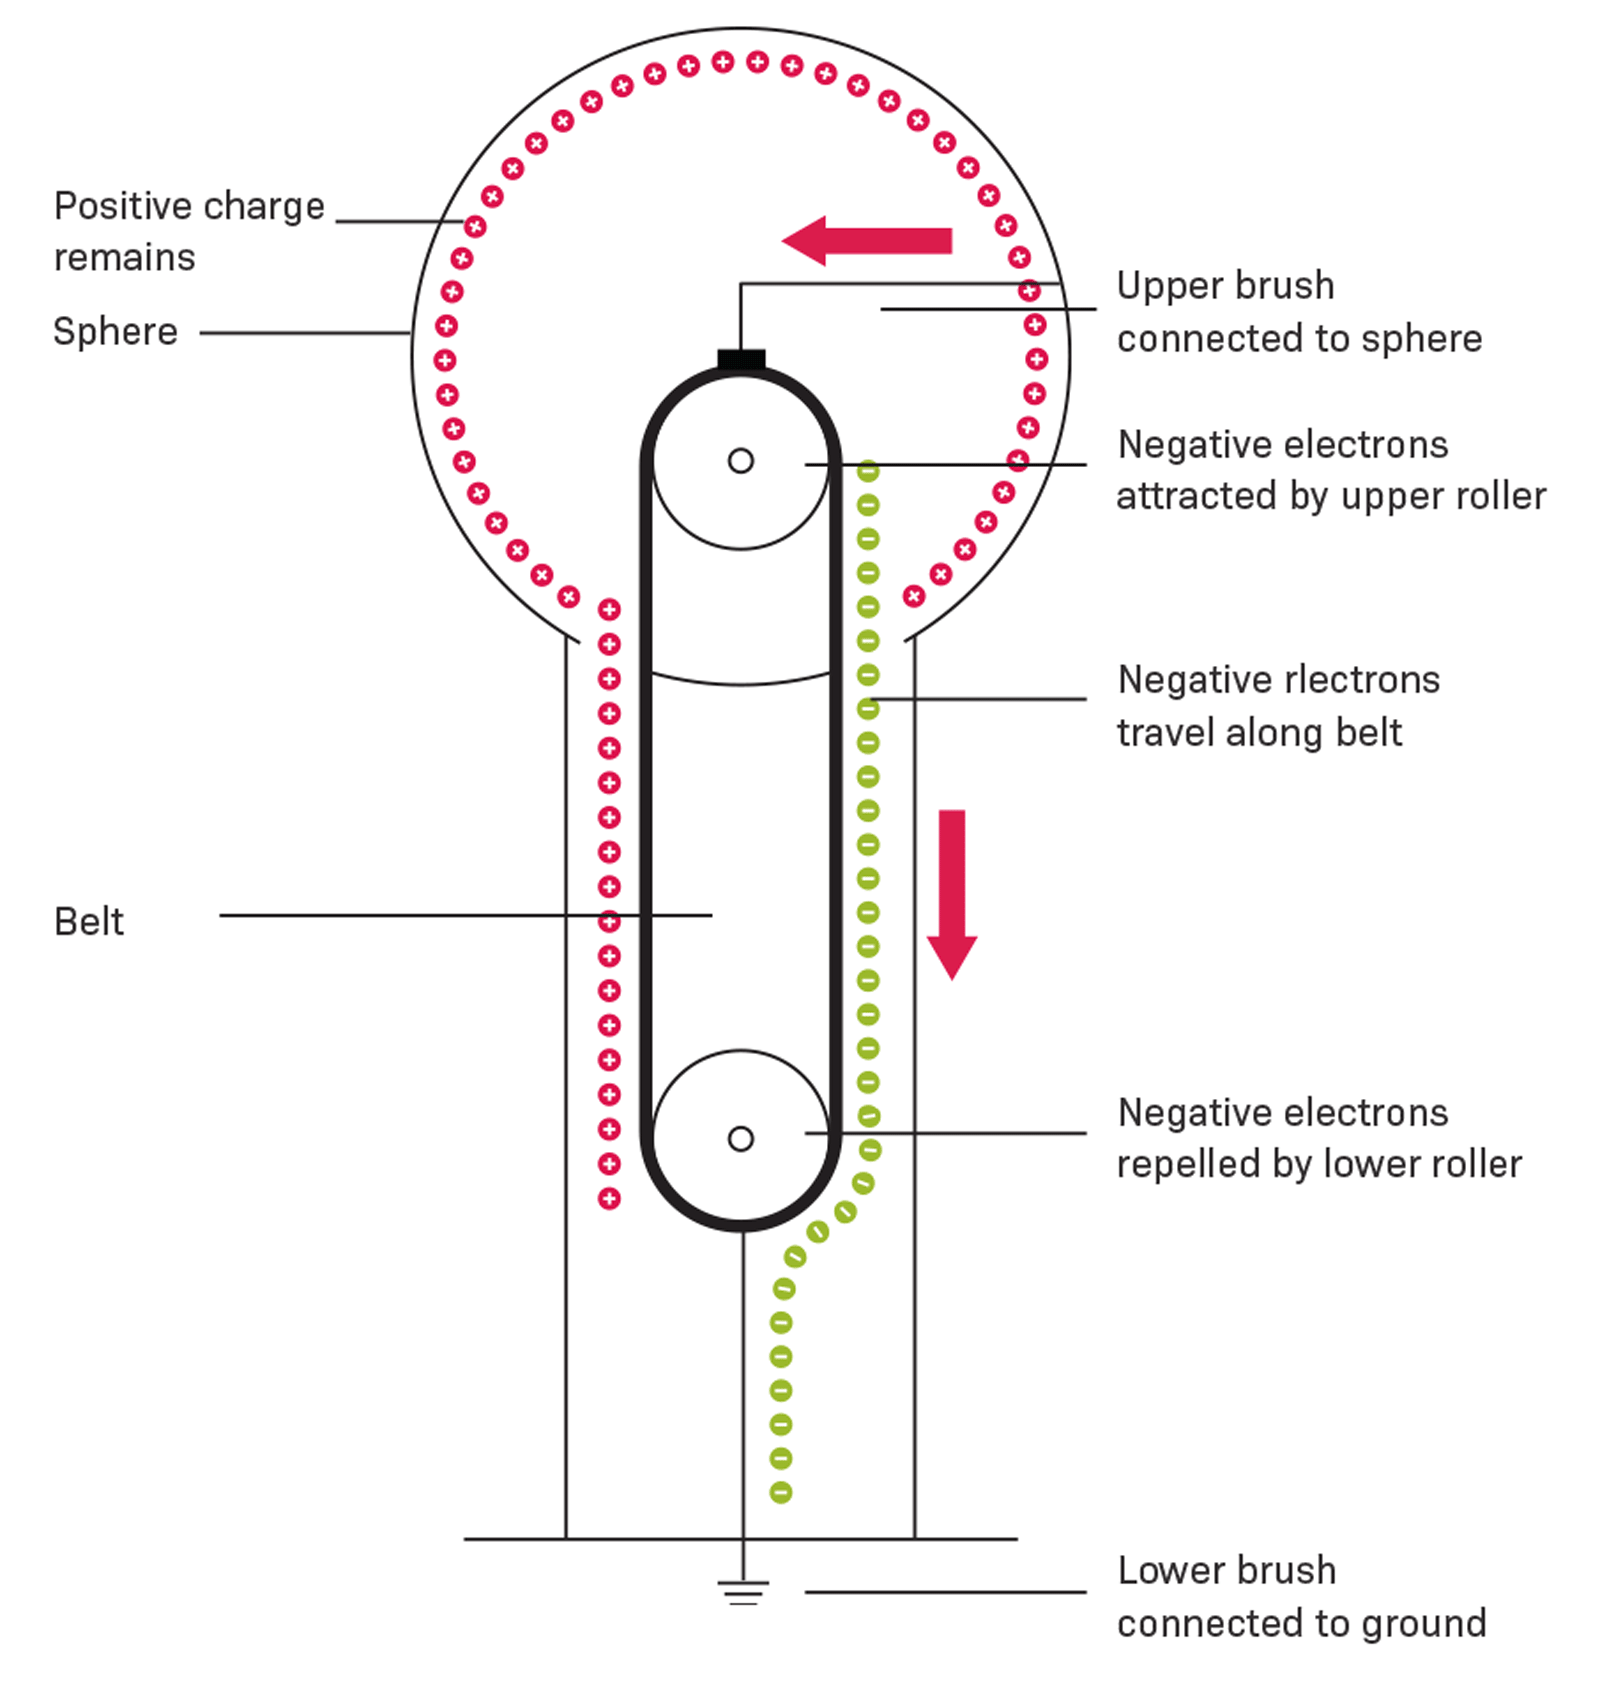
\includegraphics[width=160pt]{fig7_01}
\caption{Schema di un acceleratore di van de Graaf}
\end{figure}
L'acceleratore di Van De Graaf si compone come in figura.
La struttura è formata da una cinghia che scorre e si carica grazie a delle punte per scorrimento.
La cinghia poi passa per una sfera cava su cui viene trasferita la carica che, per i principi dell'elettrodinamica, si va a distribuire su tuttala superficie.
In questo modo si riescono a creare una differenza di potenziale dell'ordine di qualche $MeV$.
Tutto il sistema viene messo all'interno di grossi contenitori isolati in quanto l'aria farebbe scaricare le superfici (i gas inerti sostitutivi sono solitamente $SF_6, N_2+CO_2$).

Il \textbf{Tandem}, è basato sullo stesso principio del Van de Graaf, solo che la differenza di potenziale viene raddoppiata, ponendo la sfera all'interno di un altro conduttore.
\begin{figure}[h]
\centering
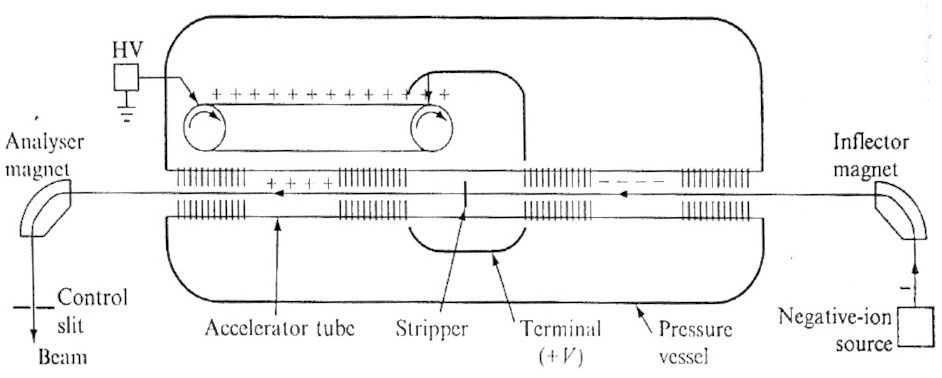
\includegraphics[width=200pt]{fig7_02}
\caption{Configurazone Tandem}
\end{figure}
Il potenziale che si riesce a creare è il doppio del potenziale di partenza.
A Legnaro è presente un acceleratore con questa configurazione e viene utilizzato per esperimenti di \emph{Rutherford backscattering}, in cui si sfrutta lo scattering del fisico neozelandese per esperimenti di spettroscopia (studiando l'energia delle particelle backscatterate si riesce a capire la composizione superficiale del bersaglio).

\paragraph{Acceleratore lineare: LINAC}
Il LINAC è stato rivoluzionario come acceleratore perché supera il limite nella generazione di potenziali.
Questo acceleratore è composto da una serie di elettrodi separati che variano la polarità con un'onda a radiofrequenza.
\begin{figure}[h]
\centering
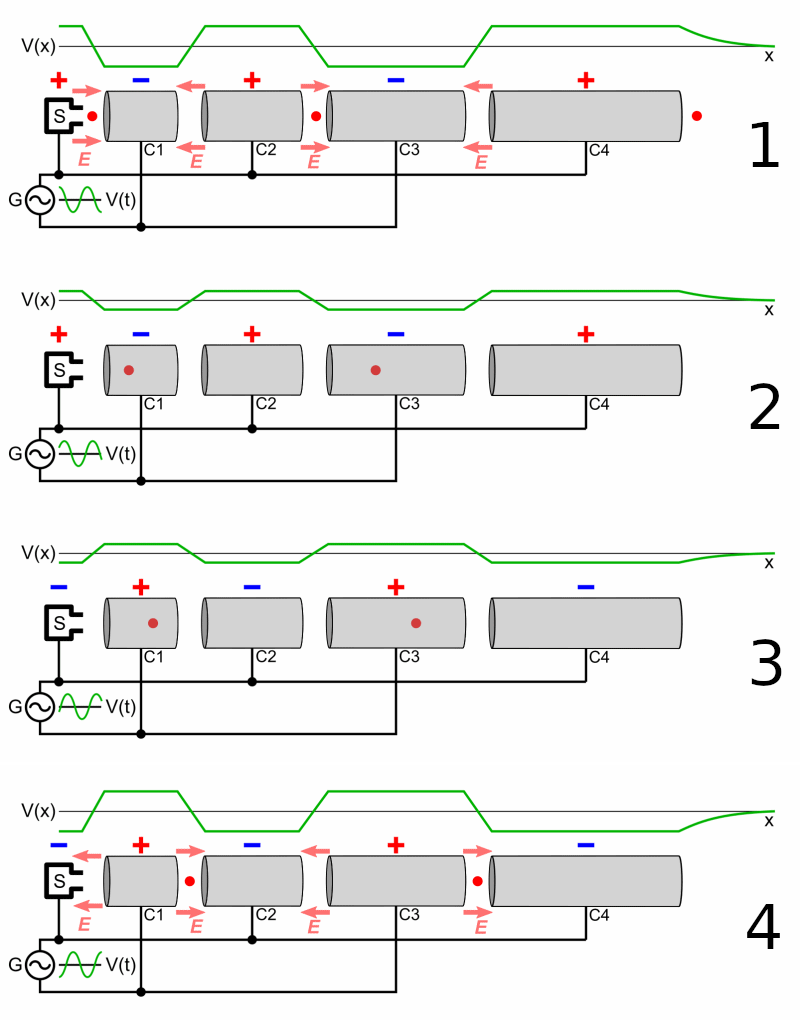
\includegraphics[width=180pt]{fig7_03}
\caption{Schema di funzionamento di un acceleratore lineare}
\end{figure}

Quello che si vuole generare con questo tipo di configurazione è un potenziale sempre negativo per la particella accelerata, infatti riuscendo a variare il potenziale al passaggio della particella, facendolo passare da positivo a negativo e viceversa, la particella nel sistema sarà sempre accelerata da un potenziale negativo rispetto a quello che ha alle sue spalle (che nel frattempo è diventato positivo).
Tutto questo fa si che pur mantenendo una differenza di potenziale piuttosto bassa si riesca ad accelerare particelle ad alte energie, questo metodo è usato per esempio per gli elettroni (in orbita circolare gli elettroni emettono radiazione).

\paragraph{Ciclotrone}
Il ciclotrone utilizza una combinazione di campi elettrici e magnetici.
Supponiamo di avere un campo magnetico entrante e di porci una particella (per esempio un protone) ciò che si crea è una forza di Lorentz, quindi a causa del campo magnetico la particella percorre una traiettoria circolare.
\begin{figure}[h]
\centering
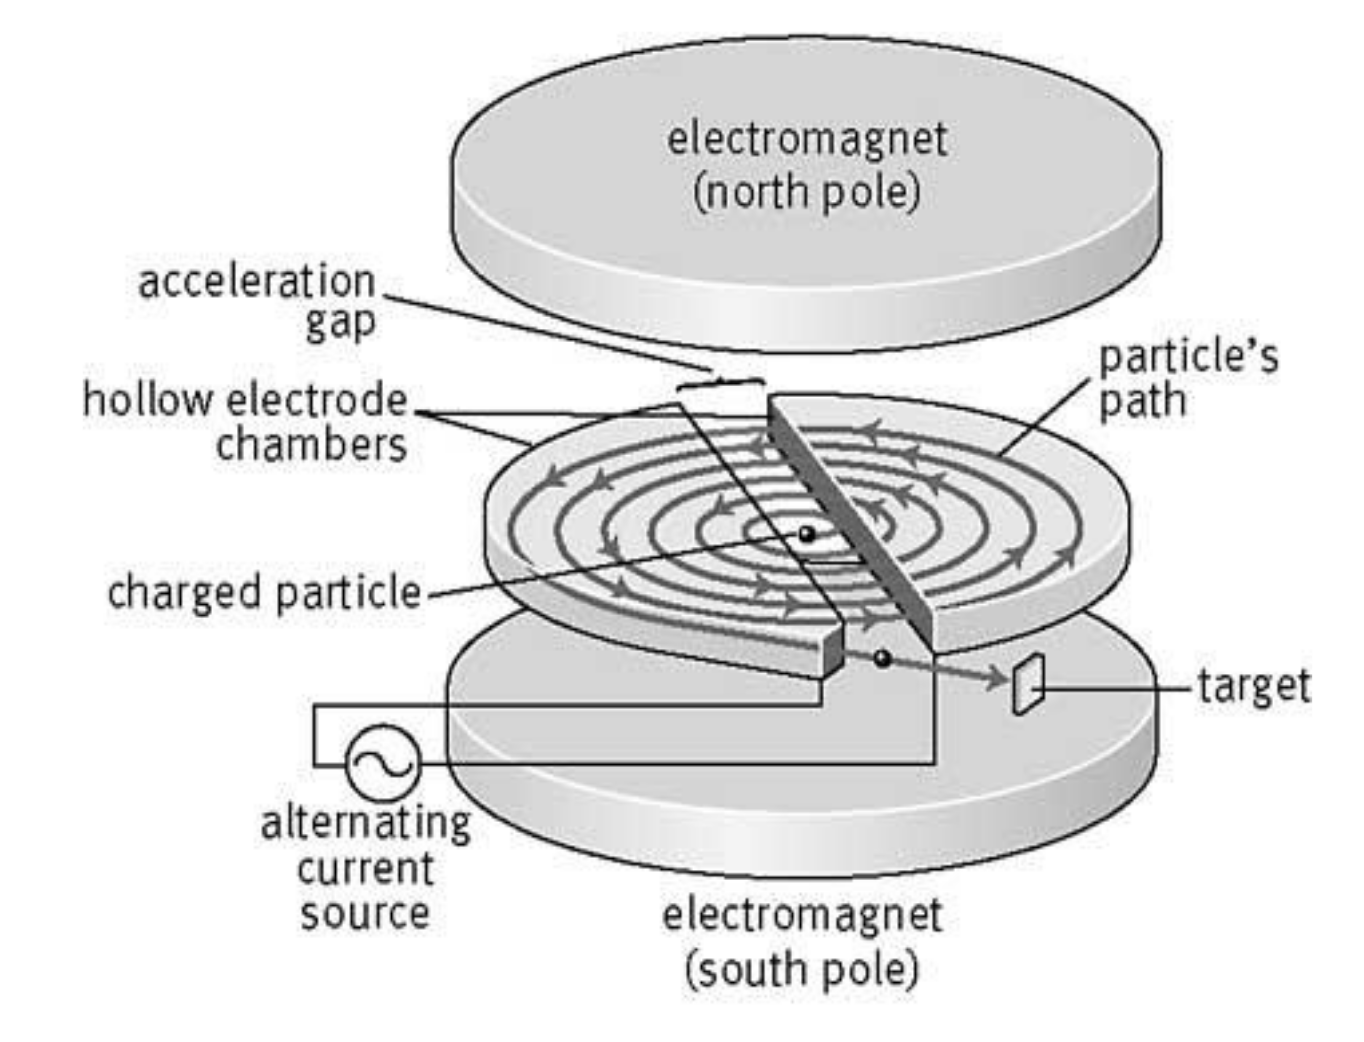
\includegraphics[width=150pt]{fig7_04}
\caption{Struttura del ciclotrone}
\end{figure}

All'interno di una situazione in cui due elettrodi hanno forma a D e sono immersi all'interno di un campo magnetico, questi vengono polarizzati uno con polarità positiva e uno con polarità negativa.
Se non si fa nulla il protone passa dal $+$ al $-$ e se cambio a polarità fa il percorso inverso.
Siccome voglio confinare la particella  applico un campo magnetico ortogonale al piano degli elettrodi.
La combinazione di campo magnetico e cambio di polarità genera un moto circolare del protone che ad ogni passaggio viene accelerato.
In questo modo si riesce ad aumentare la velocità delle particelle fino a che non raggiunge la velocità desiderata e allora posso estrarlo.

Calcoliamo le leggi che agiscono sulla particella.
Innanzitutto si ha la forza di Lorentz
\begin{equation}
F=Bqv
\end{equation}
Che corrisponde alla forza centripeta
\begin{equation}
Bqv=m\frac{v^2}{r}\to v=\frac{Bqr}{m}
\end{equation}
Calcoliamo la frequenza di variazione del campo elettrico per mantenere la particella in moto.
Il periodo di rotazione della particella è
\begin{equation}
T=\frac{2\pi r}{v}=\frac{2\pi r}{\frac{Bqr}{m}}=\frac{2\pi m}{Bq}
\end{equation}
Quindi la frequenza con cui devo variare i due elettrodi sarà
\begin{equation}
f=\frac{Bq}{2\pi m}
\end{equation}
\'E interessante notare come questa non dipenda dal raggio perché a mano a mano che la velocità aumenta la particella percorre percorsi maggiori e quindi queste due quantità si compensano.
Questo è ovviamente valido finché non si manifestano effetti relativistici sulla massa
\begin{equation}
m=m_0\cdot \gamma
\end{equation}
Esiste quindi un limite che corrisponde a qualche percentuale della velocità della luce (per esempio un protone che ha massa dell'ordine del $GeV$ può essere accelerato fino ad un massimo di $\sim 20MeV$).
